%%%%%%%%%%%%%%%%%%%%%%%%%%%%%%%%%%%%%%%%%
% Beamer Presentation
% LaTeX Template
% Version 1.0 (10/11/12)
%
% This template has been downloaded from:
% http://www.LaTeXTemplates.com
%
% License:
% CC BY-NC-SA 3.0 (http://creativecommons.org/licenses/by-nc-sa/3.0/)
%
%%%%%%%%%%%%%%%%%%%%%%%%%%%%%%%%%%%%%%%%%

%----------------------------------------------------------------------------------------
%	PACKAGES AND THEMES
%----------------------------------------------------------------------------------------

\documentclass[UTF8,aspectratio=169,14pt]{ctexbeamer}

\usepackage{hyperref}
\hypersetup{
	colorlinks=true,
	linkcolor=red,
	anchorcolor=blue,
	citecolor=green
}

\mode<presentation> {
	
	% The Beamer class comes with a number of default slide themes
	% which change the colors and layouts of slides. Below this is a list
	% of all the themes, uncomment each in turn to see what they look like.
	
	%\usetheme{default}
	%\usetheme{AnnArbor}
	%\usetheme{Antibes}
	%\usetheme{Bergen}
	%\usetheme{Berkeley}
	%\usetheme{Berlin}
	%\usetheme{Boadilla}
	%\usetheme{CambridgeUS}
	%\usetheme{Copenhagen}
	%\usetheme{Darmstadt}
	%\usetheme{Dresden}
	%\usetheme{Frankfurt}
	%\usetheme{Goettingen}
	%\usetheme{Hannover}
	%\usetheme{Ilmenau}
	%\usetheme{JuanLesPins}
	%\usetheme{Luebeck}
	\usetheme{Madrid}
	%\usetheme{Malmoe}
	%\usetheme{Marburg}
	%\usetheme{Montpellier}
	%\usetheme{PaloAlto}
	%\usetheme{Pittsburgh}
	%\usetheme{Rochester}
	%\usetheme{Singapore}
	%\usetheme{Szeged}
	%\usetheme{Warsaw}
	
	% As well as themes, the Beamer class has a number of color themes
	% for any slide theme. Uncomment each of these in turn to see how it
	% changes the colors of your current slide theme.
	
	%\usecolortheme{albatross}
	%\usecolortheme{beaver}
	%\usecolortheme{beetle}
	%\usecolortheme{crane}
	%\usecolortheme{dolphin}
	%\usecolortheme{dove}
	%\usecolortheme{fly}
	%\usecolortheme{lily}
	%\usecolortheme{orchid}
	%\usecolortheme{rose}
	%\usecolortheme{seagull}
	%\usecolortheme{seahorse}
	%\usecolortheme{whale}
	%\usecolortheme{wolverine}
	
	%\setbeamertemplate{footline} % To remove the footer line in all slides uncomment this line
	%\setbeamertemplate{footline}[page number] % To replace the footer line in all slides with a simple slide count uncomment this line
	
	%\setbeamertemplate{navigation symbols}{} % To remove the navigation symbols from the bottom of all slides uncomment this line
}

\usepackage{graphicx} % Allows including images
\graphicspath{{./figs/}}
\usepackage{booktabs} % Allows the use of \toprule, \midrule and \bottomrule in tables
\usepackage{longtable}
\usepackage{listings}
\usepackage{xcolor}
\lstset{numbers=left, %设置行号位置
	numberstyle=\tiny, %设置行号大小
	keywordstyle=\color{blue}, %设置关键字颜色
	commentstyle=\color[cmyk]{1,0,1,0}, %设置注释颜色
	frame=single, %设置边框格式
	escapeinside=``, %逃逸字符(1左面的键),用于显示中文
	%breaklines, %自动折行
	extendedchars=false, %解决代码跨页时,章节标题,页眉等汉字不显示的问题
	xleftmargin=2em,xrightmargin=2em, aboveskip=1em, %设置边距
	tabsize=4, %设置tab空格数
	showspaces=false %不显示空格
}
% Fonts
% \usepackage{libertine}
% \setmonofont{Courier}
\setCJKsansfont[ItalicFont=Noto Serif CJK SC Black, BoldFont=Noto Sans CJK SC Black]{Noto Sans CJK SC}


%----------------------------------------------------------------------------------------
%   TITLE PAGE
%----------------------------------------------------------------------------------------

\title[第7讲]{第七讲 虚拟存储:局部页面置换算法} % The short title appears at the bottom of every slide, the full title is only on the title page
\subtitle{第5节 页表自映射}
\author{向勇、陈渝} % Your name
\institute[清华大学] % Your institution as it will appear on the bottom of every slide, may be shorthand to save space
{
清华大学计算机系 \\ % Your institution for the title page
\medskip
\textit{xyong,yuchen@tsinghua.edu.cn} % Your email address
}
\date{\today} % Date, can be changed to a custom date

\begin{document}

\begin{frame}
\titlepage % Print the title page as the first slide
\end{frame}

%----------------------------------------------------------------------------------------
\begin{frame}
\frametitle{提纲} % Table of contents slide, comment this block out to remove it
\tableofcontents % Throughout your presentation, if you choose to use \section{} and \subsection{} commands, these will automatically be printed on this slide as an overview of your presentation
\end{frame}
%----------------------------------------------------------------------------------------
%   PRESENTATION SLIDES
%----------------------------------------------------------------------------------------
%------------------------------------------------
\section{第5节 页表自映射}% Sections can be created in order to organize your presentation into discrete blocks, all sections and subsections are automatically printed in the table of contents as an overview of the talk
%------------------------------------------------
\subsection{页表自映射} % A subsection can be created just before a set of slides with a common theme to further break down your presentation into chunks
%------------------------------------------------
% ### 页表自映射
%------------------------------------------------
\begin{frame}
    \frametitle{基于4KB页面的32位CPU二级页表}
    \begin{figure}
    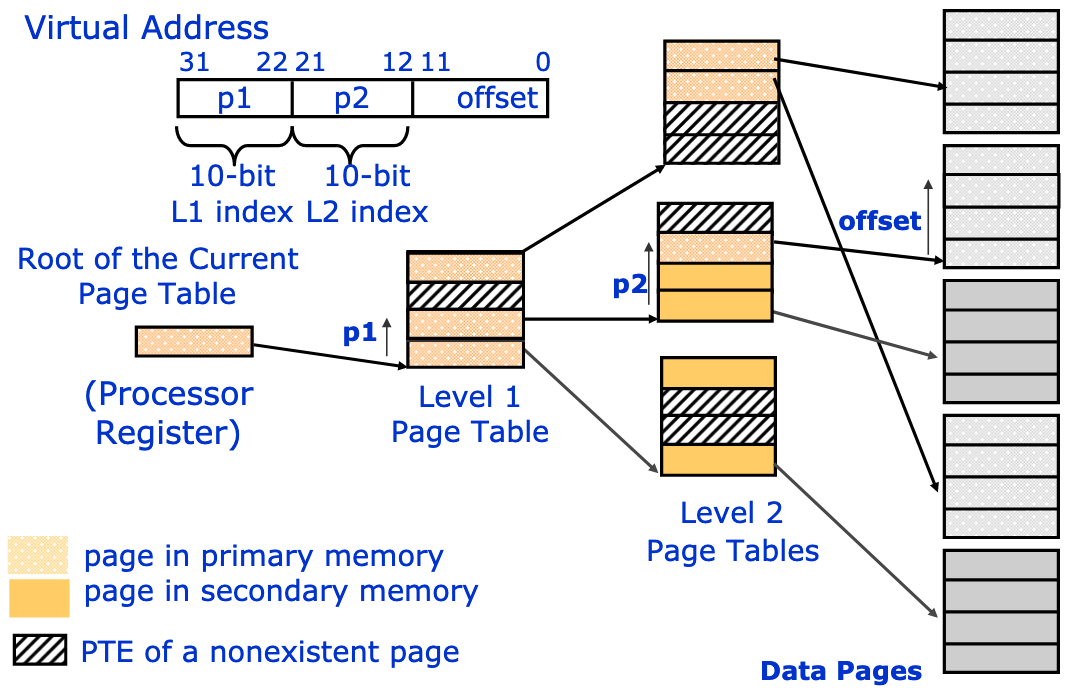
\includegraphics[width=0.7\linewidth]{figs/2-level-pagetable.png}
%    \caption{xxxx}
    \end{figure}
\end{frame}
%------------------------------------------------

% #### 基于4KB页面的32位CPU二级页表
% 
% https://cseweb.ucsd.edu/classes/wi14/cse141/pdf/08/12_CSE141-MBT-Virtual-Memory.ppt.pdf
% 
% Page 8:
% 
% ![2-level-pagetable](figs/2-level-pagetable.png)
%------------------------------------------------
\begin{frame}
    \frametitle{地址转换的计算过程}
    \begin{figure}
    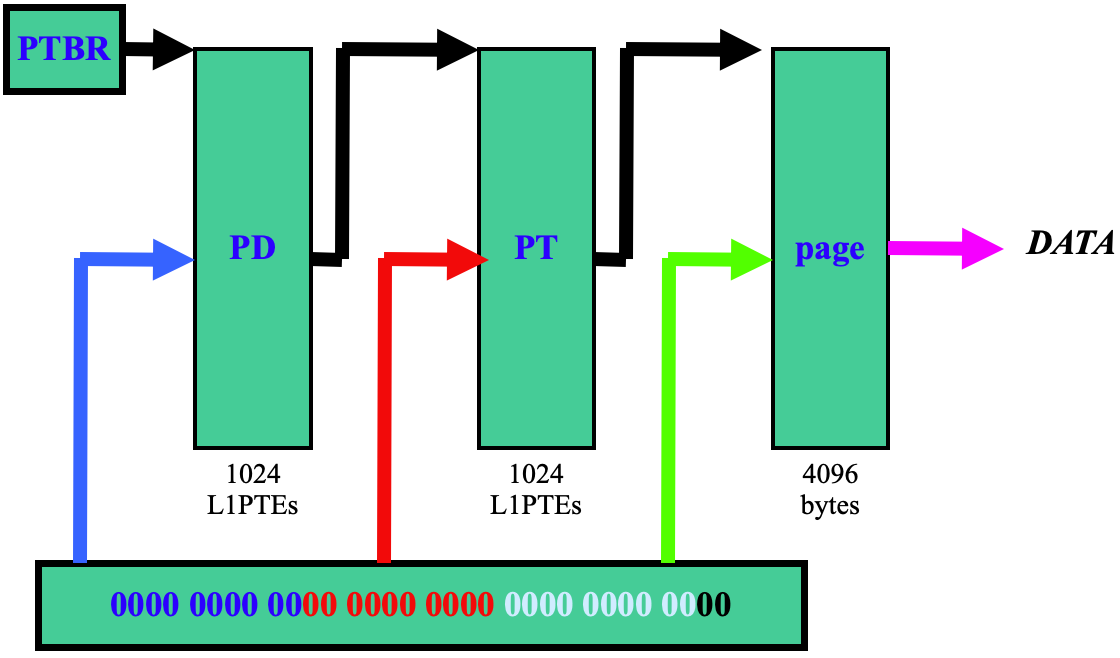
\includegraphics[width=0.75\linewidth]{figs/addr-translation.png}
%    \caption{xxxx}
    \end{figure}
\end{frame}
%------------------------------------------------
% #### 地址转换的计算过程
% 
% 20130326-lecture05-mm-instance.pptx
% Page 10
% 
% 计算过程图
% 
% ![addr-translation](figs/addr-translation.png)
%------------------------------------------------
\begin{frame}
    \frametitle{页表自映射机制}
    \begin{figure}
    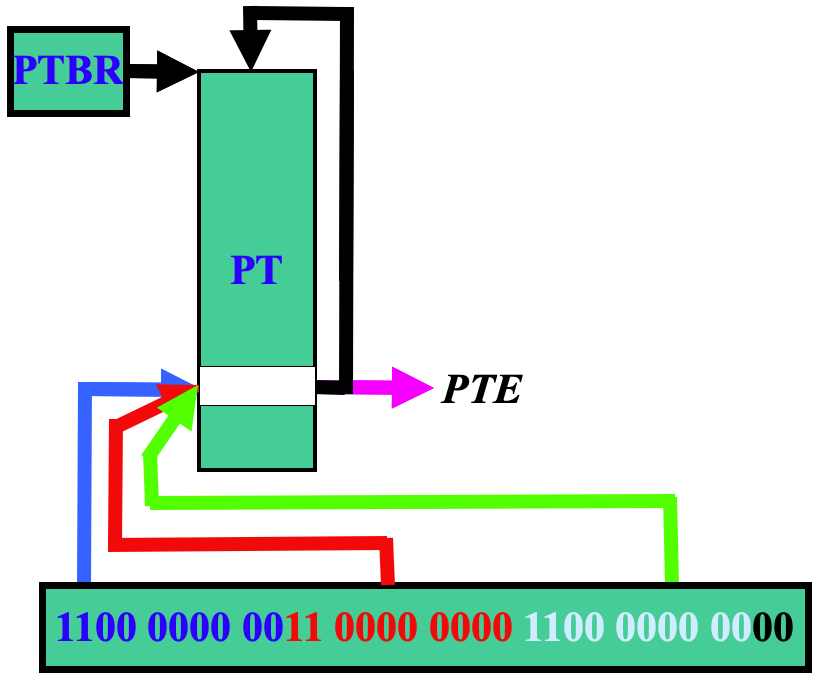
\includegraphics[width=0.55\linewidth]{figs/self-mapping-PTE.png}
%    \caption{xxxx}
    \end{figure}
\end{frame}
%------------------------------------------------
% #### 页表自映射机制
% 
% ![self-mapping-PTE](figs/self-mapping-PTE.png)
%------------------------------------------------
\subsection{X86-32页表自映射} % A subsection can be created just before a set of slides with a common theme to further break down your presentation into chunks
%------------------------------------------------
% ### X86-32页表自映射

%------------------------------------------------
\begin{frame}
    \frametitle{基于4KB页面的X86-32二级页表}
    \begin{figure}
    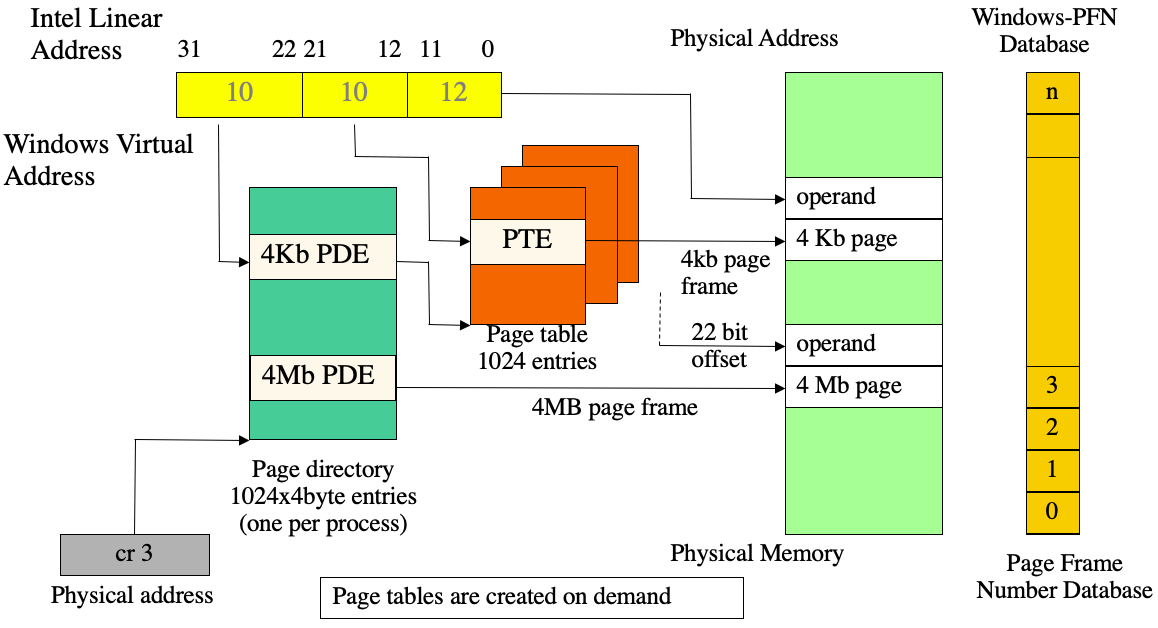
\includegraphics[width=0.8\linewidth]{figs/x86-32-addr-translation.png}
%    \caption{xxxx}
    \end{figure}
\end{frame}
%------------------------------------------------
% #### 基于4KB页面的X86-32二级页表
% 
% 20130326-lecture05-mm-instance.pptx
% Page 9
% 
% 地址转换和二级页表的
% 
% ![x86-32-addr-translation](figs/x86-32-addr-translation.png)
%------------------------------------------------
\begin{frame}
    \frametitle{X86-32页表项结构}
    \begin{figure}
    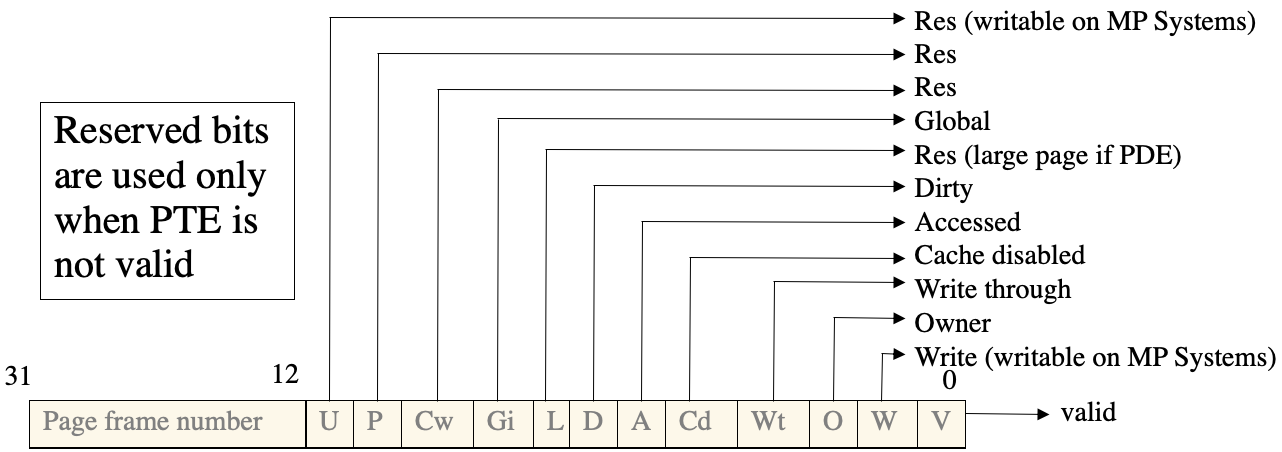
\includegraphics[width=0.8\linewidth]{figs/x86-32-page-tabel-entry.png}
%    \caption{xxxx}
    \end{figure}
\end{frame}
%------------------------------------------------
% #### X86-32页表项结构
% 
% Ref: 20130326-lecture05-mm-instance.pptx
% Page 17
% 
% ![x86-32-page-tabel-entry](figs/x86-32-page-tabel-entry.png)
%------------------------------------------------
\begin{frame}[fragile,plain]
    \frametitle{用C语言宏表示的地址转换中虚拟地址字段获取}
    \begin{block}{}
    \begin{verbatim}
// page directory index
#define PDX(la) ((((uintptr_t)(la)) >> PDXSHIFT) & 0x3FF)
// page table index
#define PTX(la) ((((uintptr_t)(la)) >> PTXSHIFT) & 0x3FF)
// page number field of address
#define PPN(la) (((uintptr_t)(la)) >> PTXSHIFT)
// offset in page
#define PGOFF(la) (((uintptr_t)(la)) & 0xFFF)
    \end{verbatim}
    \end{block}
\end{frame}
%------------------------------------------------
% #### 用C语言宏表示的地址转换计算过程
% 
% 20130326-lecture05-mm-instance.pptx
% Page 11
% 
% ```c
% // page directory index
% #define PDX(la) ((((uintptr_t)(la)) >> PDXSHIFT) & 0x3FF)
% // page table index
% #define PTX(la) ((((uintptr_t)(la)) >> PTXSHIFT) & 0x3FF)
% // page number field of address
% #define PPN(la) (((uintptr_t)(la)) >> PTXSHIFT)
% // offset in page
% #define PGOFF(la) (((uintptr_t)(la)) & 0xFFF)
% ```
%------------------------------------------------
\begin{frame}
    \frametitle{X86-32的第一级页表的自映射}
    \begin{figure}
    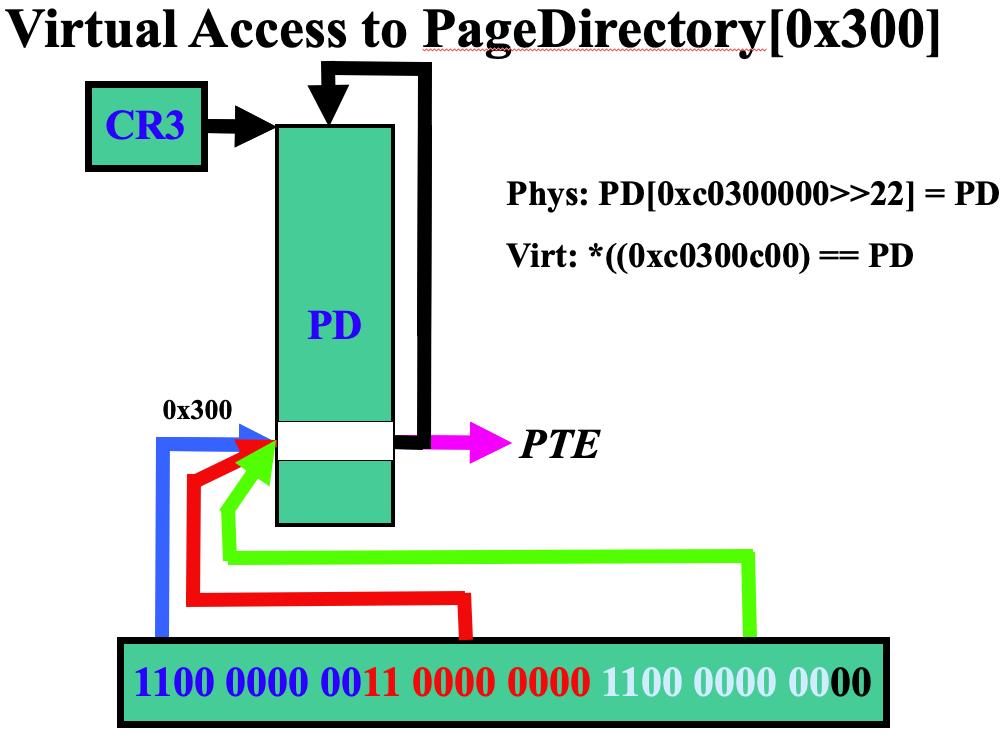
\includegraphics[width=0.63\linewidth]{figs/1-level-self-mapping-pt.png}
%    \caption{xxxx}
    \end{figure}
\end{frame}
%------------------------------------------------
% #### X86-32的第一级页表的自映射
% 20130326-lecture05-mm-instance.pptx
% Page 23
% 
% ![1-level-self-mapping-pt](figs/1-level-self-mapping-pt.png)
%------------------------------------------------
\begin{frame}
    \frametitle{X86-32的第二级页表的自映射}
    \begin{figure}
    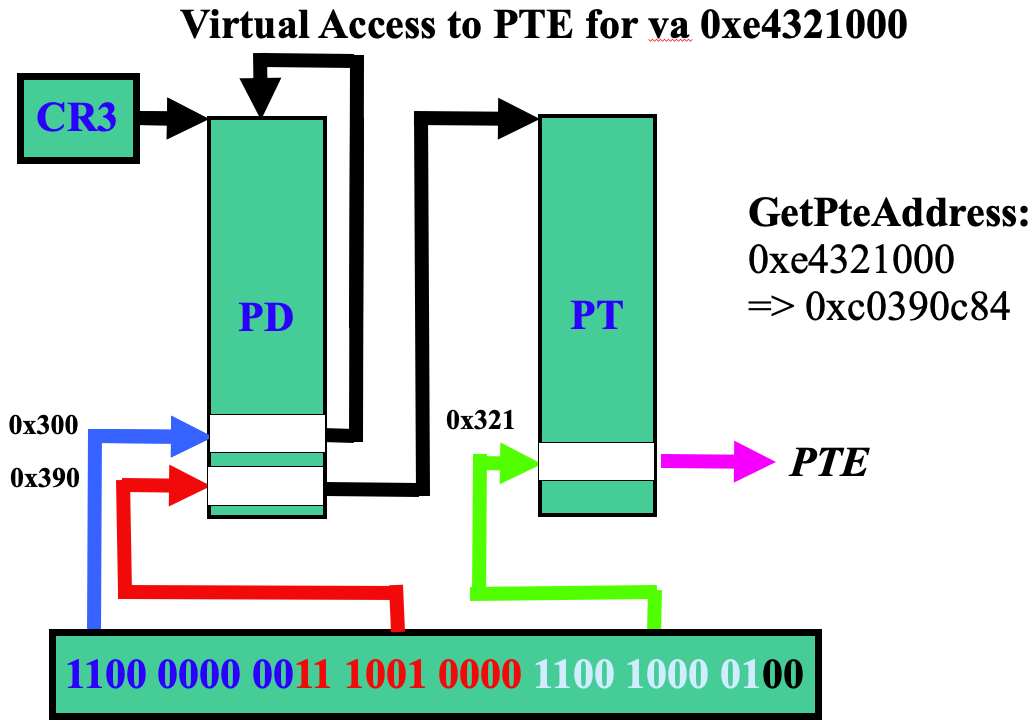
\includegraphics[width=0.63\linewidth]{figs/2-level-self-mapping-pt.png}
%    \caption{xxxx}
    \end{figure}
\end{frame}
%------------------------------------------------
% #### X86-32的第二级页表的自映射
% 20130326-lecture05-mm-instance.pptx
% Page 24
% 
% ![2-level-self-mapping-pt](figs/2-level-self-mapping-pt.png)
%------------------------------------------------
\begin{frame}[fragile,plain]
    \frametitle{X86-32自映射页表项初始化}
%% C Code
    \begin{block}{}
    \begin{verbatim}
//C CODE
// recursively insert boot_pgdir in itself
// to form a virtual pate table at virtual address VPT
boot_pgdir[PDX(VPT)] = PADDR(boot_pgdir) | PTE_P | PTE_W;
    \end{verbatim}
    \end{block}
\end{frame}
%------------------------------------------------
% #### X86-32自映射页表项初始化
% ```C
% // recursively insert boot_pgdir in itself
% // to form a virtual pate table at virtual address VPT
% boot_pgdir[PDX(VPT)] = PADDR(boot_pgdir) | PTE_P | PTE_W;
% ```
%------------------------------------------------
\subsection{riscv32页表自映射} % A subsection can be created just before a set of slides with a common theme to further break down your presentation into chunks
%------------------------------------------------
% ### riscv32页表自映射
%------------------------------------------------
\begin{frame}
    \frametitle{RISC-V Sv32二级页表}
    \begin{figure}
    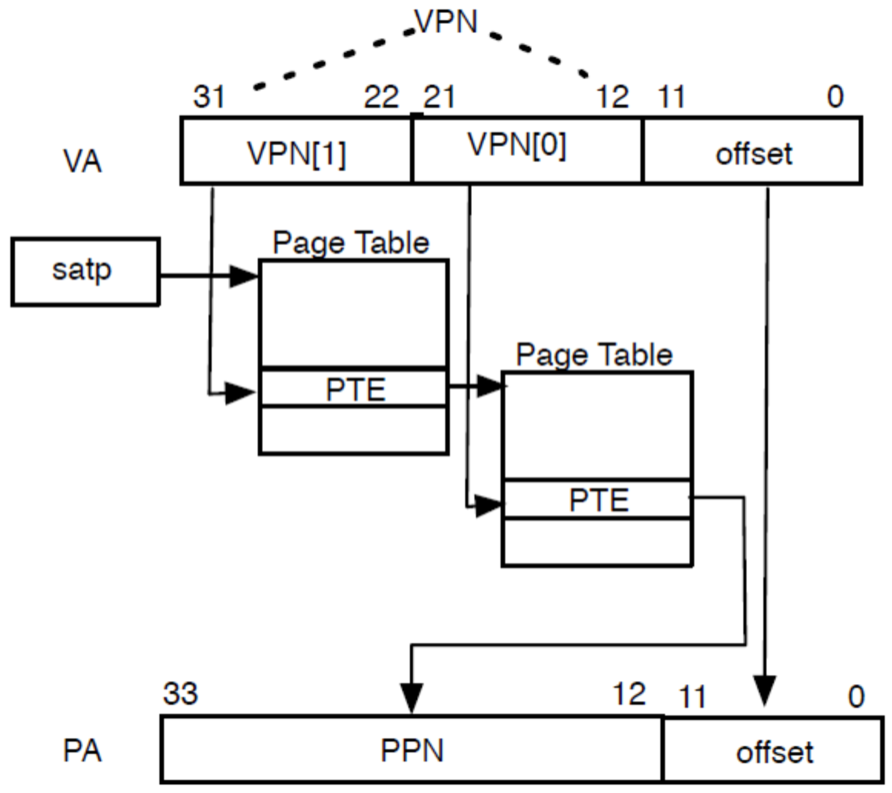
\includegraphics[width=0.5\linewidth]{figs/riscv32-pagetable.png}
%    \caption{xxxx}
    \end{figure}
\end{frame}
%------------------------------------------------
% #### RISC-V Sv32的二级页表

% https://learningos.github.io/rcore_step_by_step_webdoc/docs/%E9%A1%B5%E8%A1%A8%E7%AE%80%E4%BB%8B.html
% 图
% 
% ![riscv32-pagetable](figs/riscv32-pagetable.png)
%------------------------------------------------
\begin{frame}
    \frametitle{RISC-V32页表项结构:Sv32页表项格式}
        \begin{figure}
        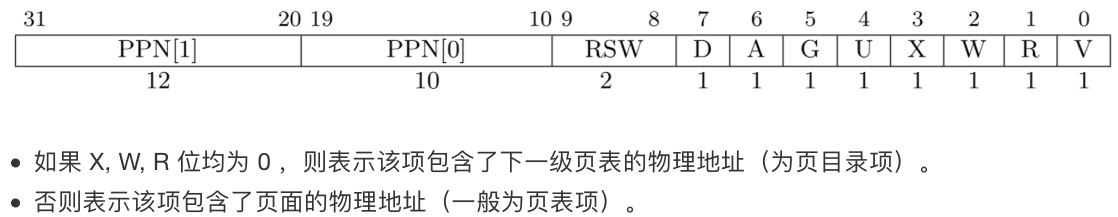
\includegraphics[width=1.0\linewidth]{figs/riscv32-page-entry.png}
    %    \caption{xxxx}
        \end{figure}
\end{frame}
%------------------------------------------------
\begin{frame}
    \frametitle{RISC-V32页表项结构:页表项R/W/X字段含义}

        \begin{figure}
        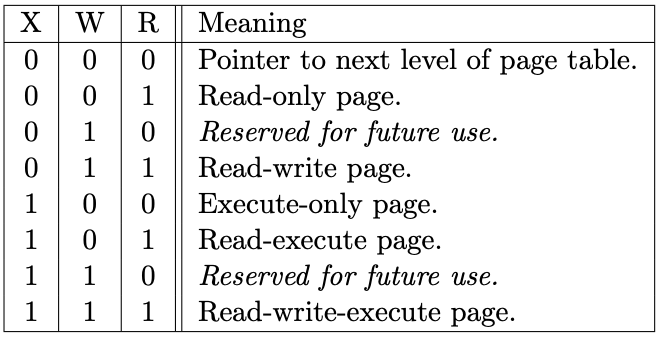
\includegraphics[width=0.9\linewidth]{figs/PTE-RWX-fields.png}
    %    \caption{xxxx}
        \end{figure}

\end{frame}
%------------------------------------------------
% #### RISC-V32页表项结构
% 
% Ref: https://learningos.github.io/rcore_step_by_step_webdoc/docs/页表简介.html
% riscv-privileged-20190608-1.pdf
% Page 80:
% Figure 4.15: Sv32 page table entry
% 
% ![riscv32-page-entry](figs/riscv32-page-entry.png)
% 
% riscv-privileged-20190608-1.pdf
% Table 4.4: Encoding of PTE R/W/X fields.
% 
% ![PTE-RWX-fields](figs/PTE-RWX-fields.png)
%------------------------------------------------
\begin{frame}
    \frametitle{rCore中riscv-Sv32自映射}

%% columns
    \begin{columns}
    \begin{column}{0.6\textwidth}
        \begin{figure}
        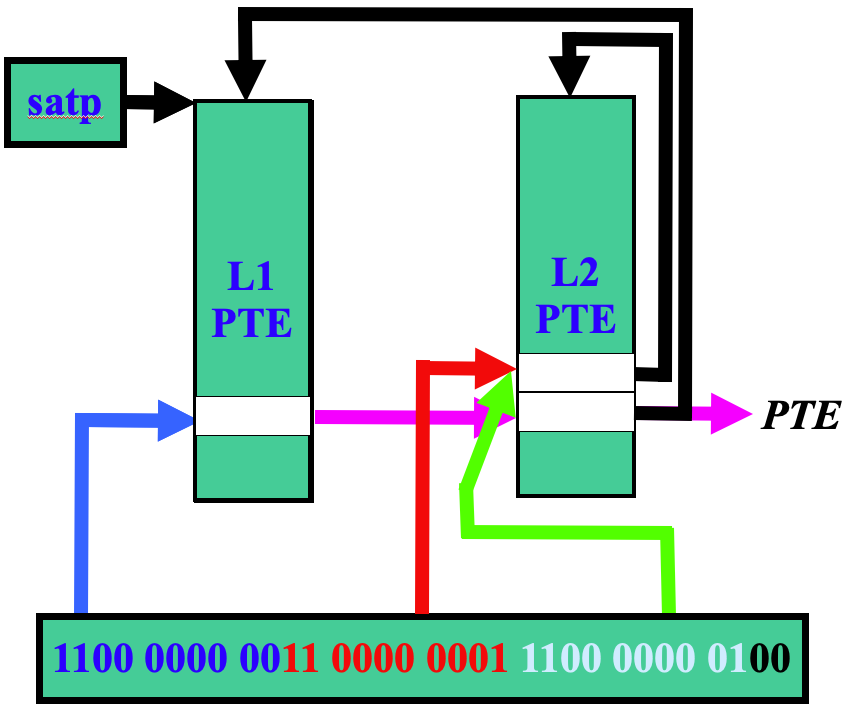
\includegraphics[width=0.9\linewidth]{figs/riscv32-self-mapping.png}
    %    \caption{xxxx}
        \end{figure}
    \end{column} \pause
    \begin{column}{0.4\textwidth}
        \begin{itemize}
            \item RISCV页表项中的flags,明确表示它指向的是数据页(VRW),还是下层页表(V)。
            \item 在访问一级页表虚地址期间,将它所对应的二级页表项flags置为VRW。
            \item 访问二级页表本身,还需要再加一个自映射的二级页表项,其flags为VRW。
        \end{itemize}
    \end{column}
    \end{columns}

\end{frame}
%------------------------------------------------
% #### rCore中riscv-Sv32自映射
% 
% /Users/xyong/github/rCore/docs/1_OS/RISCV.md
% 
% ![riscv32-self-mapping](figs/riscv32-self-mapping.png)
% 
% RISCV页表项中的flags,明确表示它指向的是数据页(VRW),还是下层页表(V)。
% 在访问一级页表虚地址期间,将它所对应的二级页表项flags置为VRW。
% 访问二级页表本身,还需要再加一个自映射的二级页表项,其flags为VRW。
%------------------------------------------------
\end{document}
